\documentclass[12pt]{article}
\usepackage{amsmath, amssymb, graphicx, hyperref}
\usepackage{indentfirst}
\title{Plasma Mirrors}
\author{Harikesh}
\date{\today}

\newenvironment{changemargin}[2]{%
\begin{list}{}{%
\setlength{\topsep}{0pt}%
\setlength{\leftmargin}{#1}%
\setlength{\rightmargin}{#2}%
\setlength{\listparindent}{\parindent}%
\setlength{\itemindent}{\parindent}%
\setlength{\parsep}{\parskip}%
}%
\item[]}{\end{list}}
\begin{document}
\begin{titlepage}
    \begin{changemargin}{-2cm}{-2cm}
        \begin{figure}
            
\includegraphics[width=5cm, height=5cm]{logo.png}
            \centering
        \end{figure}
        \begin{center}
            \textbf{\Large{Department of Physics, IIT Delhi}}\\
            \vspace*{1cm}
            \textbf{\Large{Course Code : PYD561}}\\
            \vspace*{0.2cm}
            \textbf{\Large {Semester - III, 2022-23}}\\
            \vspace*{1cm}
            \textbf{\LARGE{Plasma Mirrors}}\\
            \vspace*{1cm}
            \textbf{\Large{Kulwinder Kaur (2021PHS7190)}}\\
            \vspace*{0.2cm}
            \textbf{\Large {Harikesh Kushwaha (2021PHS7181)}}\\
            \vspace*{1cm}
            \textbf{\Large {Adviser: Prof. Vikrant Saxena}}\\
            \vspace*{2cm}
        \end{center}
        \begin{flushleft}


            \textbf{Signature of student 1: \ldots \ldots \ldots}\\
            \vspace*{1cm}
            \textbf{Signature of student 2: \ldots \ldots \ldots}
            \hspace*{3cm}
            \textbf{Signature of the adviser: \ldots \ldots \ldots}
        \end{flushleft}
    \end{changemargin}
\end{titlepage}
\newpage
\begin{changemargin}{-3cm}{-3cm}
    \section{Introduction And Motivation}
    Interaction of relativistic and non-relativistic laser pulse is studied with underdense and overdense plasma. Underdense plasma is transparent to the laser pulse while overdense plamsa is opaque and reflects the laser back.
    In case of relativistic laser pulse, the plasma frequency gets shifted and hence the pulse passes through the plasma even though the plasma was underdense to start with.

    When a laser pulse is incident upon plasma, it reflects if the density of plasma is large enough, forming a plasma mirror (PM). Upon reflection from the plasma the laser field drives relativistic oscillation of the PM surface due to pondermotive force that induces a periodic temporal compression of the reflected field through the Doppler effect. These oscillations results in generation of high harmonics of the incident laser frequency.\cite{lichters}


    \section{Methodology}
    The simulation uses \textit{epoch}, a parallised, second order and fully relativistic implementation of particle in cell (PIC) algorithm.\cite{epoch} Though \textit{epoch} is implemented in 3D, the current simulation is performed in 1D3V only.
    \subsection{PIC Algorithm}
    In plasma physics, the PIC method is a numerical approach that simulates a collection
    of charged particles that interact via external and self-induced electromagnetic fields. A
    spatial grid is used to describe the field while the particles move in the continuous space. The field and the particle motion are solved concurrently. In this case the simulation
    requires less amount of work, since each particle only interacts with the grid points of
    the cell where it is located.\cite{suciu}

    % \newpage
    % \noindent

    \subsection{Underdense and Overdense Plasma}
    Plasma frequency for plasma density $n_p$ is given by\cite{chen}
    \begin{equation}\label{plasma-frequency}
        \omega_p = \sqrt{\frac{n_p e^2}{\epsilon_0 m_e}}
    \end{equation}
    If the frequency of the incident laser pulse, $\omega_l$, is greater than the plasma frequency, the plasma is called underdense. In this case, the plasma is transparent to the laser pulse. On the other hand, if the frequency of the incident laser pulse is less than the plasma frequency, the plasma is called overdense. In this case, the laser can not penetrate the plasma deeply and is reflected back. The case $\omega_l = \omega_p$ corresponds to critical plasma and density in this case is called critical density $n_c$. Using Equation \hyperref[plasma-frequency]{1} gives;
    \begin{equation}\label{critical-density}
        n_c = \frac{\epsilon_0 m_e \omega_l^2}{e^2}
    \end{equation}
    % The skin depth of the plasma is given by
    % \begin{equation*}
    %     \delta = \frac{c}{\omega_p}
    % \end{equation*}
    \subsection{Laser Pulse}
    The simulation uses ultrashort laser pulses. An ultrashort laser emitts pulse with duration of the order of pico second. Defining the laser vector potential as $$ a_0 = \frac{eE_0}{m w_l c}$$
    A laser is called relativistic if $a_0 \ge 1$.

    \subsection{Parameters for Simulation}
    The simulation box extends for $20 \lambda _l$ (from $-10 \lambda _l$ to $10 \lambda _l$), where $\lambda_l$ is the laser wavelength and has total 1000 cells. The plasma is placed at $x=0$ and with a thickess of $\lambda_l$. Number of particles per cell are 100.  The plasma density $n_p$ is defined in terms of the critical density $n_c$ and is varied from 0.1 to 10. The vector potential $a_0$ of the laser pulse is also varied as 0.1, 1.0 and 10 for each set of plasma density.

    The envelope of the incident laser field varies according to
    \begin{equation}\label{envelope}
        P(t)=
        \begin{cases}
             & \sin^2(\pi t/T) \text{ for } 0 \leq t \le T \\
             & 0         \;      \text{ otherwise }
        \end{cases}
    \end{equation}
    Where T is the pulse duration here taken as $T=10\tau$ with $\tau = 2\pi/\omega_l$ is the time of one laser cycle. The simulation is performed for $t=20\tau$.
    \section{Result and Discussion}
    Reflecatance here is define as

    \begin{equation}\label{reflectance}
        R
        = \frac{{E_{300}^2}-{E_{600}^2}}{{E_{300}^2}}
    \end{equation}
    where $E_{300}$ is the sum of y component of the electric field at $300^{th}$ node and $E_{600}$ is the sum of y component of the electric field at $600^{th}$ node for all the simulation time. The plot of reflectance with different ratio of $n_c$ and $n_0$ is shown in the figure below for different values of vector potential $a_0$.

    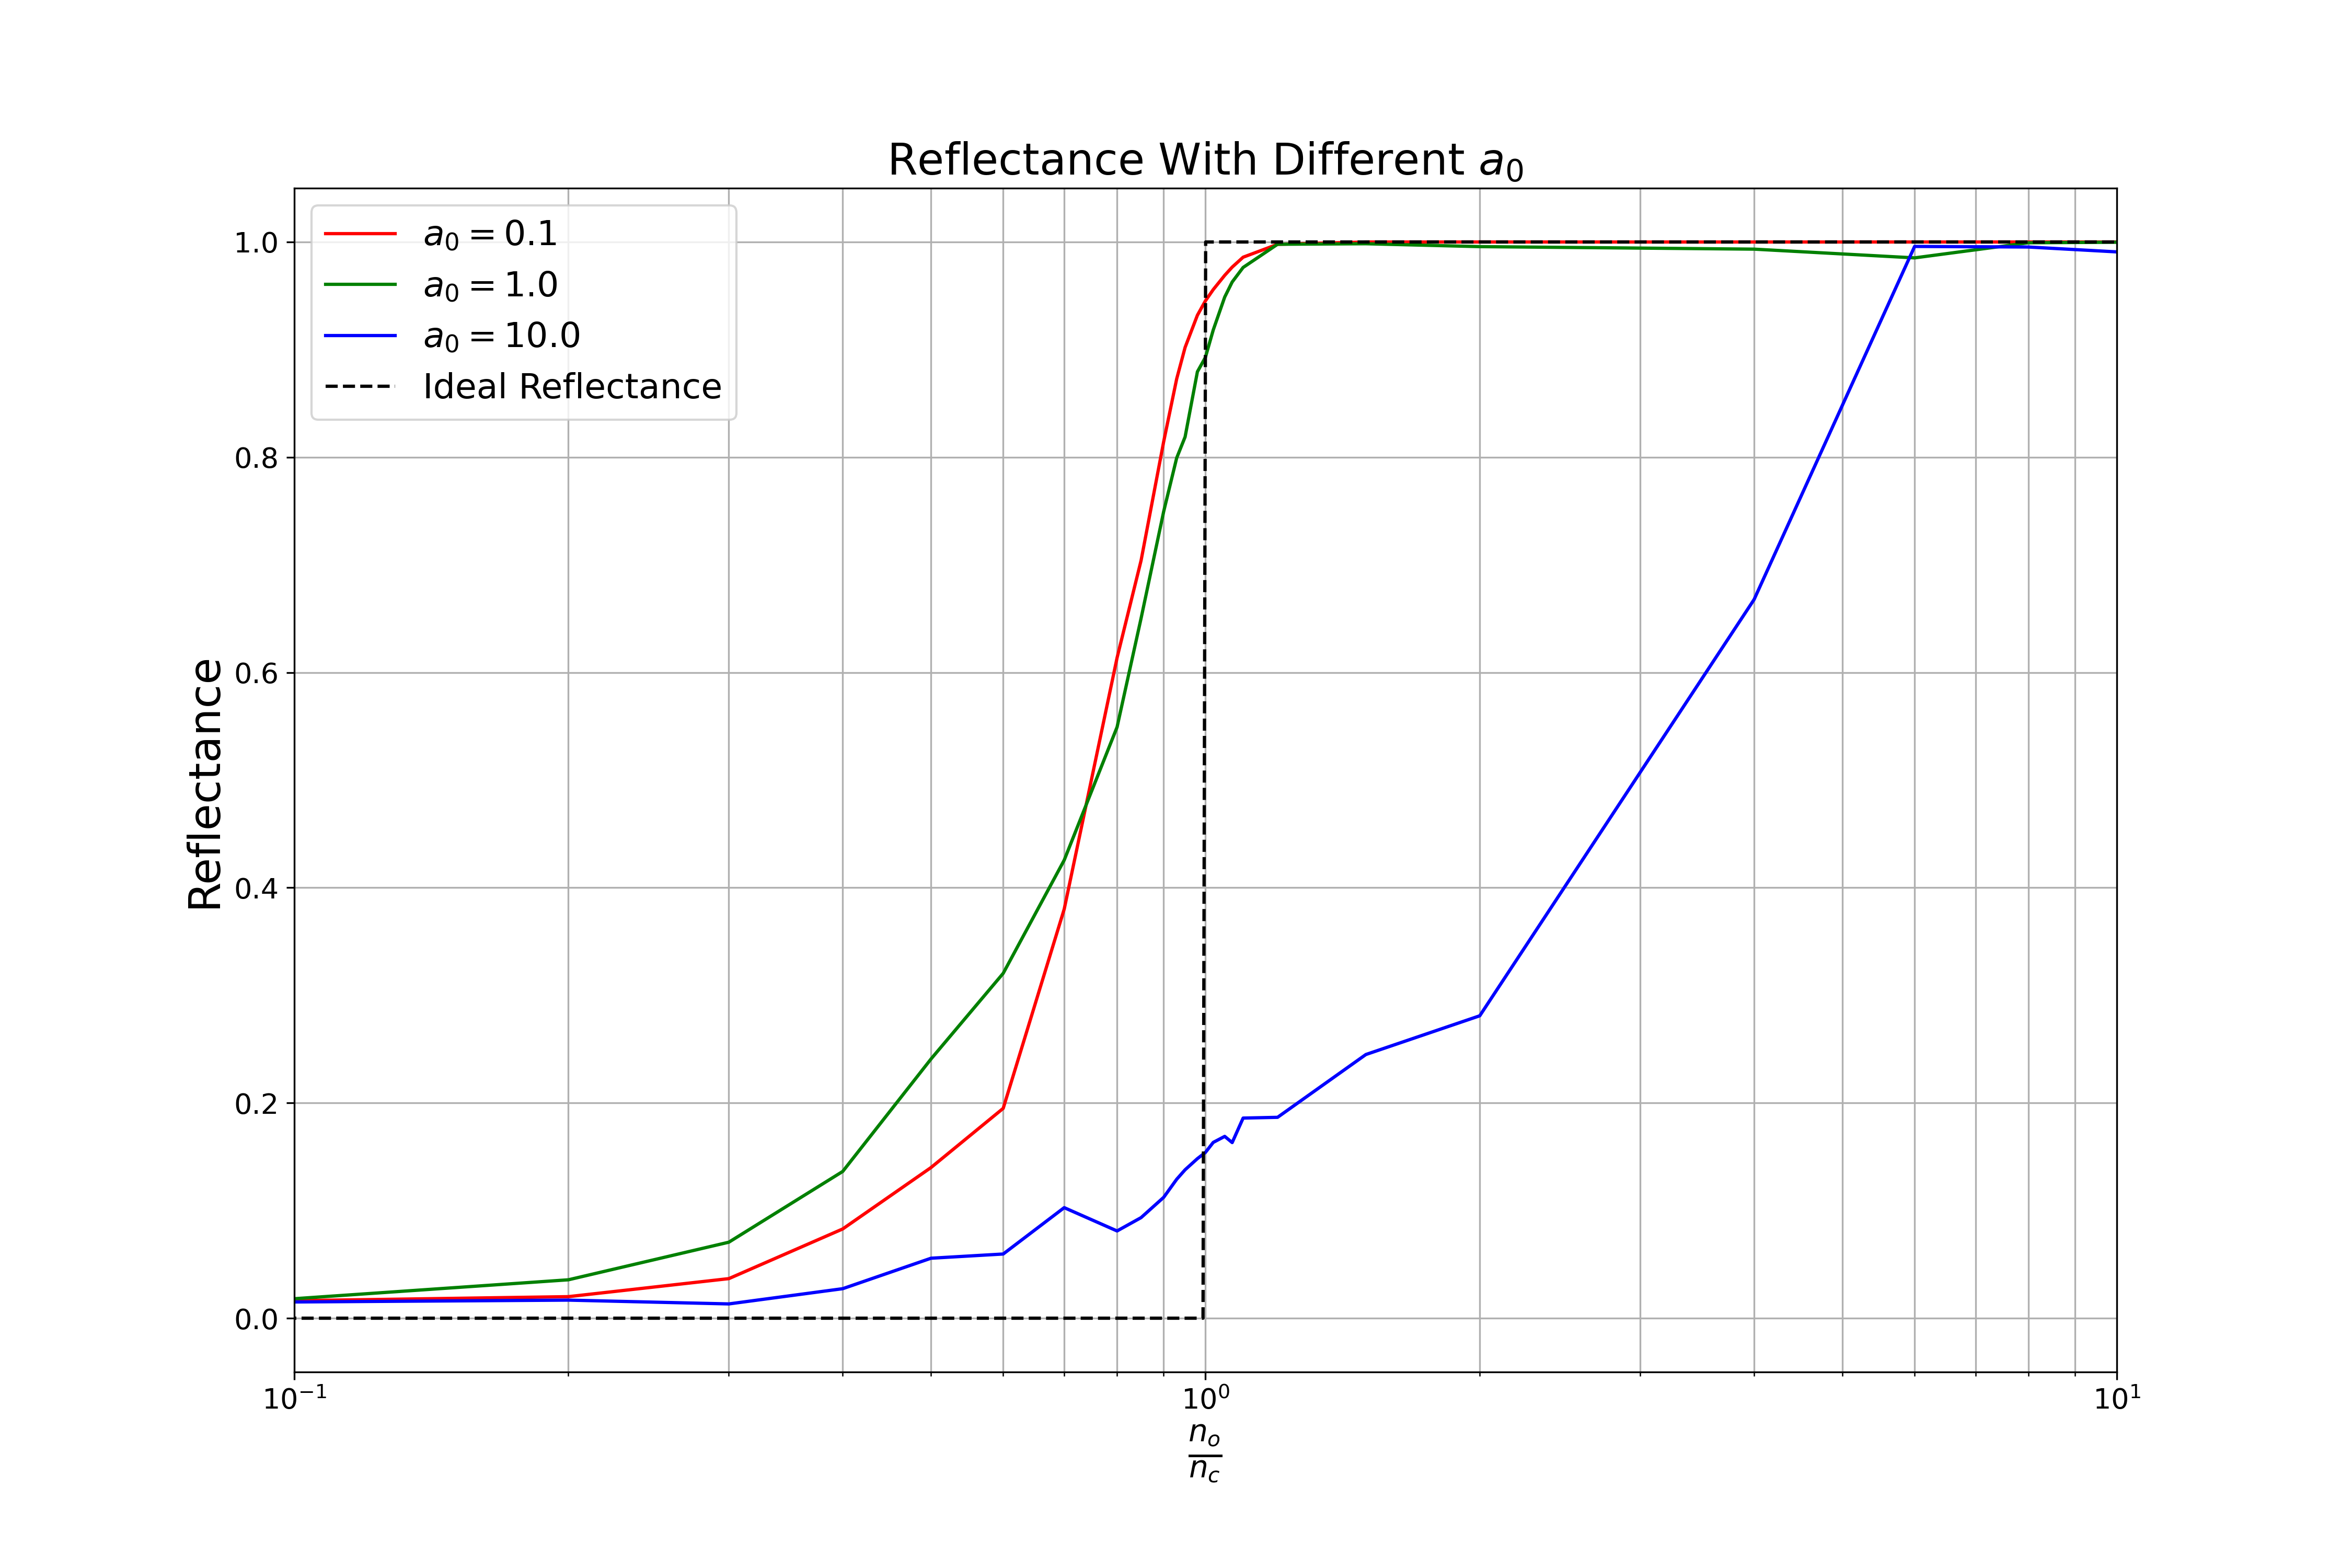
\includegraphics[width=20cm, height=13cm]{reflection.png}
    \begin{center}
        Plot of reflectance (see \hyperref[reflectance]{4}) with different ratio of $n_c$ and $n_0$ for different values of vector potential $a_0$.
    \end{center}
    \vspace*{0.2cm}
    The ideal curve for the interaction of laser pulse with underdense and overdense plasma is shown in the figure with black dotted line. Ideally, when the ration $r = \frac{n_0}{n_c}$ becomes 1, the reflectance should also become 1. However, when the laser becomes relativistic for $a_0 \ge 1$, the particles inside plasma starts to oscillate with relativistic velocity, gaining mass. This results in change in the plasma frequency and hence the laser does not get reflected even for density greater than the critical density corresponding to the non-relativistic case. So, there is a shift in the critical density due to relativistic laser pulse.

    Next, the plot of the oscillation of plasma surface with time is shown for different values of vector potential. The laser pulse, after interacting with electrons, makes them oscillate. If the pulse becomes relativistic, the oscillations becomes strong and hence the plasma surface oscillates with relativistic velocity.
    The figure below shows that for $a_0=0.1$, the oscillation is very weak. As $a_0$ increases, the oscillation becomes stronger.
    \noindent
    \begin{center}
        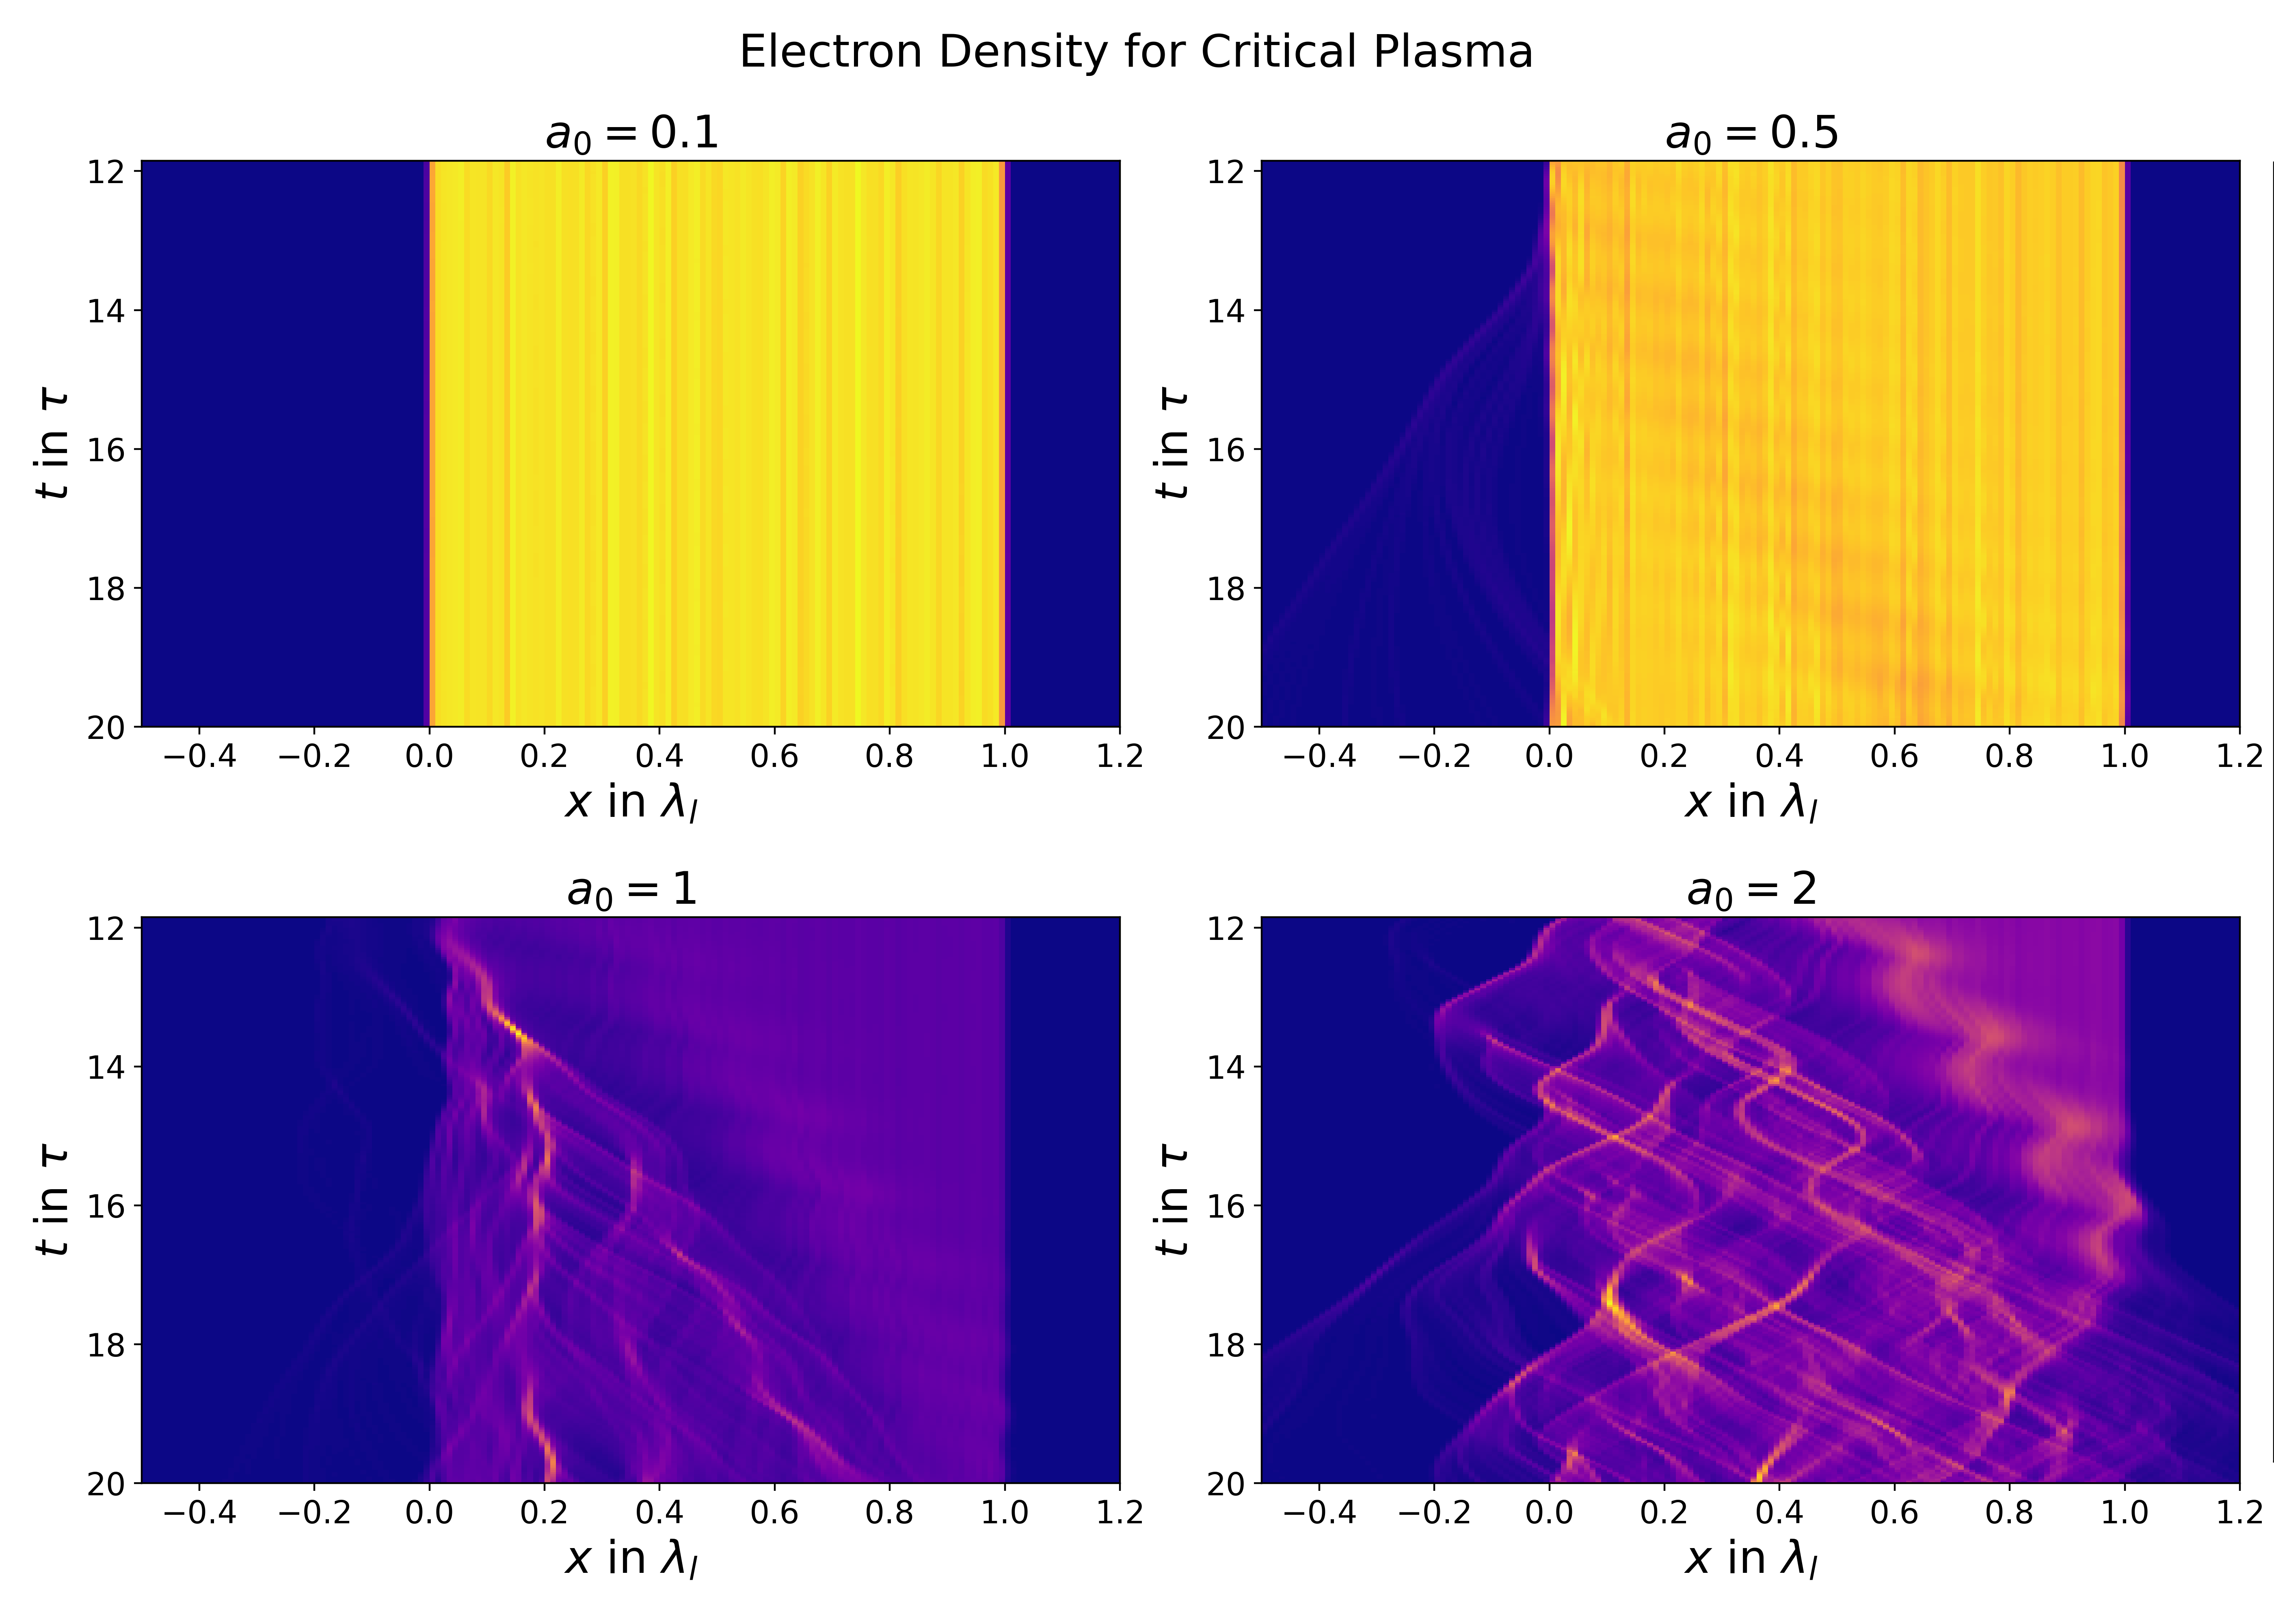
\includegraphics[height=9cm, width=16cm]{density.png}

    \end{center}
    \section{Current Status and Future Plan of Work}
    Study of interaction of relativistic and non-relativistic laser pulse is studied with underdense and overdense plasma. Future plan is simulation of harmonic generation in 1D using ultrashort intense laser pulse.
    \section{Acknowledgement}
    We are very thankful to Prof. Vikrant Saxena for his support and valuable guidance.
    \begin{thebibliography}{9}
        \bibitem{lichters}
        R. Lichters Et al. Physics of Plasmas 3, pp. 3425-3437 (1996)

        \bibitem{epoch}
        Arber, T D Et al. Plasma Physics and Controlled Fusion 57 1-26 (2015)

        \bibitem{suciu}
        Alin Suciu Et al. 2020 15th Conference on Computer Science and Information Systems (FedCSIS), pp.381-385, 2020

        \bibitem{chen}
        Francis F. Chen
        Introduction to Plasma Physics and Controlled Fusion $3^{rd}$ Ed.

    \end{thebibliography}

\end{changemargin}
\end{document}